\section{Cognacy Queries Over Dependence Graphs}
\label{sec:conjugate}

We now turn to cognacy and ``co-cognacy'' queries over dependence graphs, expressed in terms of the
$\demandsR$ and $\demandedByR$ operators introduced informally in \secref{overview}. Boolean algebras
(\defref{conjugate:Boolean-algebra}) are used to represent selections; we then define $\demandsR$ and
$\demandedByR$ and their De Morgan duals, first for an arbitrary relation (\secref{conjugate:image-preimage})
and then for the \emph{IO relation} of a dependence graph (\secref{conjugate:dependence-graph-functions}).
Then we give procedures for computing $\demandsR$ and $\demandedByR$ and their duals over a given dependence
graph, via an intermediate graph slice (\secref{conjugate:dependence-graph-algos}).

\begin{definition}[Boolean algebra]
\label{def:conjugate:Boolean-algebra}
A \emph{Boolean algebra} (or \emph{Boolean lattice}) $A$ is a 6-tuple $(A, \meet, \join, \bot, \top, \neg)$
with carrier $A$, distinguished elements $\bot$ (bottom) and $\top$ (top), commutative operations $\meet$
(meet) and $\join$ (join) with $\top$ and $\bot$ as respective units, and unary operation $\neg$ (negate)
satisfying $x \join \neg x = \top$ and $x \meet \neg x = \bot$. The operations $\meet$ and $\join$ distribute
over each other and induce a partial order $\leq$ over $X$.
\end{definition}

An input (or output) selection, where $X$ is the set of all addresses that occur in the input (or output) of
the program, is represented by the \emph{powerset} Boolean algebra $\powerset{X}$ whose carrier is the set of
subsets $X' \subseteq X$ ordered by inclusion $\subseteq$. In this case bottom is the empty set $\emptyset$,
top is the whole set $X$, meet and join are given by $\cap$ and $\cup$, and negation by relative complement
$\setminus$, so that $\neg X' = X \setminus X'$.

\subsection{$\demandsR$ and $\demandedByR$ and their duals}
\label{sec:conjugate:image-preimage}

A mnemonic device may now help: imagine program outputs at the top and inputs at the bottom;
\emph{demanded by} $\demandedByR$ `expands downwards' from outputs (top) to
     those inputs (bottom) demanded by those outputs;
\emph{demands} $\demandsR$ `expands upwards' from inputs (bottom) to those outputs (top) which demand those inputs.

The $\demandsR$ and $\demandedByR$ operators sketched earlier are simply the image and preimage functions for
a particular relation $R$.

\begin{definition}[Image and Preimage Functions for a Relation]
   For a relation $R \subseteq X \times Y$, define $\demandedByR_R: \powerset{X} \to \powerset{Y}$ and
   $\demandsR_R : \powerset{Y} \to \powerset{X}$ as:
   \begin{enumerate}
      \item $\demandedByR_{R}(X') \eqdef \set{y \in Y \mid \exists x \in X'.(x,y) \in R}$ \hfill (image)
      \item $\demandsR_{R}(Y') \eqdef \set{x \in X \mid \exists y \in Y'. (x,y) \in R}$ \hfill (preimage)
   \end{enumerate}
\end{definition}

\noindent Trivially $\demandedByR_{R} = \demandsR_{R^{-1}}$. The image and preimage functions form a
\textit{conjugate pair}, in the sense of \citet{jonsson51}:

\begin{definition}[Conjugate Functions]
   For Boolean algebras $A$, $B$, functions $f: A \to B$ and $g: B \to A$ form a \textit{conjugate pair} iff:
   $$
   f(x) \meet y = \bot \iff x \meet g(y) = \bot
   $$
\end{definition}

% \noindent (\citet{jonsson51} consider only endofunctions; here we extend the idea of conjugacy to maps
% between Boolean algebras.)

\begin{lemma}
\label{lem:im-preim-conjugate}
$\demandedByR_{R}$ and $\demandsR_{R}$ are conjugate.
\end{lemma}

This should be intuitive enough: for any subsets $X' \subseteq X$ and $Y' \subseteq Y$, if the elements ``on
the right'' to which $X'$ is related are disjoint from $Y'$, then there are no edges in $R$ from $X'$ to $Y'$;
and in virtue of that, the elements ``on the left'' to which $Y'$ is related must also be disjoint from $X'$.

Conjugate functions are related to another class of near-reciprocals between Boolean algebras, namely
\emph{Galois connections}; in fact every conjugate pair induces a Galois connection~\cite{menni14}. This
relates the present setting to previous work on program slicing with Galois
connections~\cite{perera12a,perera16d,ricciotti17}.

\begin{definition}[Galois connection]
   \label{def:conjugate:galois-connection}
   Suppose $A, B$ are partial orders, then monotone functions $f: A \to B$ and $g: B \to A$ form a \textit{Galois
   connection} iff
   \[ f(x) \leq y \iff x \leq g(y) \]
\end{definition}

\begin{proposition}%[Correspondence Between Conjugates and Galois Connections]
   \label{prop:conj-galois-correspond}
   Suppose functions $f: A \to B$ and $g: B \to A$ between Boolean algebras. The following statements are
   equivalent:
   \begin{enumerate}
      \item $f$ and $g$ form a conjugate pair
      \item $f$ and $\dual{g}$ form a Galois connection
   \end{enumerate}
\end{proposition}
%
It is also useful (both for performance reasons and as a user feature) to consider the \emph{De Morgan duals}
of $\demandsR$ and $\demandedByR$, which we write as $\sufficesR$ and $\preimageDualR$; these also form a
conjugate pair.

\begin{definition}[De Morgan Dual]
   \label{def:conjugate:de-morgan-dual}
   Suppose a function $f: A \to B$ between Boolean algebras with $\neg_A$ and $\neg_B$ the negation operators
   of $A$ and $B$. Define the \textit{De Morgan Dual} $\dual{f}: A \to B$ of $f$ as:
   \[ \dual{f} \eqdef \neg_B \after f \after \neg_A \]
\end{definition}

\begin{definition}[Dual Image and Preimage Functions for a Relation]
   For relations $R \subseteq X \times Y$, define $\sufficesR_R: \powerset{X} \to \powerset{Y}$ and
   $\preimageDualR_R: \powerset{Y} \to \powerset{X}$ as:
   \begin{enumerate}
      \item $\sufficesR_R(X') \eqdef \set{y \in Y \mid \nexists x \in X \setminus X'.(x, y) \in R}$ \hfill
      (dual image)
      \item $\preimageDualR_R(Y') \eqdef \set{x \in X \mid \nexists y \in Y \setminus Y'.(x, y) \in R}$ \hfill
      (dual preimage)
   \end{enumerate}
\end{definition}
%
Bearing in mind that $\neg$ for $\powerset{X}$ is just relative complement $X \setminus \param$, it is easy to
show that these are indeed the intended De Morgan duals.

\begin{lemma}[Duality of image and preimage functions]
   \label{lem:conjugate:image-preimage-duality}
   \item
   \begin{enumerate}
      \item $\dual{\demandedByR_R} = \sufficesR_R$
      \item $\dual{\demandsR_R} = \preimageDualR_R$
   \end{enumerate}
\end{lemma}

\noindent If $\demandedByR_R(X')$ picks out the outputs that the elements of $X'$ are \emph{necessary} for,
$\sufficesR_R(X')$ picks out the outputs that the elements of $X$ are \emph{sufficient} for.
$\preimageDualR_R(Y')$ picks out the inputs that are needed \emph{only} by elements of $Y'$.

% \noindent (Taking the opposite graph has the effect of swapping sources and sinks.)

\subsection{$\demandsR_G$ and $\demandedByR_G$ for Dependence Graphs}
\label{sec:conjugate:dependence-graph-functions}

%\subsubsection{IO Relation for a Graph}

Reachability in $G$ induces a relation just between \emph{sources} and \emph{sinks}, which we call the
\emph{IO} relation of $G$. We now extend $\demandsR_{R}$ and $\demandedByR_{R}$ and their duals to a
dependence graph $G$, via its IO relation.

\begin{definition}[Sources and sinks]
For a graph $G = (V,E)$, write $\sources{G}$ for the \emph{sources} of $G$ (i.e.~those vertices with no
in-edges) and $\sinks{G}$ for the \emph{sinks} of $G$ (those with no out-edges).
\end{definition}

\begin{definition}[Reachability relation]
Define the \emph{reachability relation} for a graph $G=(V,E)$ to be the reflexive transitive closure of $E$.
\end{definition}

\begin{definition}[IO relation]
For any dependence graph $G$ with reachability relation $R$, define the \emph{IO} relation of $G$ to be $R
\cap (\sources{G} \times \sinks{G})$.
\end{definition}

The IO relation specifies how specific inputs (sources) are demanded by specific outputs (sinks); thus we
interpret $(x, y) \in R$ as ``$x$ is \textit{demanded by} $y$''. Clearly the IO relation of $G$ is the
converse of the IO relation of $\opGraph{G}$. The set of inputs that some outputs $Y$ \emph{demand},
$\demandsR_{G}(Y)$, is simply the subset of the inputs of $G$ reachable from $Y$ (by traversing the graph in
its opposite direction). Conversely, the set of outputs \emph{demanded by} some inputs $X$,
$\demandedByR_{G}(X)$, is simply the subset of the outputs of $G$ reachable from $X$.

% Since we are in fact interested in the relationship between
% input and output \emph{selections} (namely sets of inputs and outputs), we now consider how such a relation $R
% \subseteq X \times Y$ lifts to $\powerset{X}$ and $\powerset{Y}$ via the \textit{image} and \textit{preimage}
% functions for $R$, which we will denote using $\demandedByR_{R}$ and $\demandsR_{R}$.

\begin{definition}[$\demandsR_G$ and $\demandedByR_G$ for a dependence graph]
   For a graph $G$ with IO relation $R$, define:
   \begin{enumerate}
      \item $\demandsR_G \eqdef \demandsR_{R}: \powerset{\sinks{G}} \to \powerset{\sources{G}}$ \hfill
      (demands)
      \item $\demandedByR_G \eqdef \demandedByR_{R}: \powerset{\sources{G}} \to \powerset{\sinks{G}}$ \hfill
      (demanded by)
   \end{enumerate}
\end{definition}

\subsection{Computing $\demandsR_G$, $\demandedByR_G$, $\sufficesR_{G}$ and $\preimageDualR_{G}$ for
Dependence Graphs}
\label{sec:conjugate:dependence-graph-algos}

We now show how to compute e$\demandsR_{G}$, $\demandedByR_{G}$, $\sufficesR_{G}$ and $\preimageDualR_{G}$ for
a dependence graph $G$, via an intermediate graph slice which we then restrict to its IO relation. First some
graph notation:

\begin{definition}[In-edges and out-edges]
For a graph $G=(V,E)$ and vertex $\alpha \in V$, write $\inE{G}(\alpha)$ for the in-edges of $\alpha$ in $G$
and $\outE{G}(\alpha)$ for its out-edges.
\end{definition}

\begin{definition}[Opposite graph]
For a graph $G$ define the \emph{opposite} graph $\opGraph{G} \eqdef (V,E^{-1})$ where $\param^{-1}$ denotes
relational converse.
\end{definition}

With the trace-based approaches mentioned in \secref{introduction}, one can use a given algorithm to implement
its De Morgan dual; for example, given a procedure for $\demandedByR_{G}$ we can compute $\sufficesR_{G}$ by
pre- and post-composing with negation~\cite{perera22}. In the dependence graph setting, we can also use a given
algorithm to compute its conjugate, e.g., given a procedure for $\demandedByR_{G}$, we can compute
$\demandsR_{G}$ simply as $\demandedByR_{\opGraph{G}}$.

For efficiency, however, we give direct procedures both for $\demandedByR_{G}$
(\secref{conjugate:algorithm:demandedBy}) and $\sufficesR_{G}$ (\secref{conjugate:algorithm:suffices}), which
can then be used to derive implementations of the other operators, as shown at the end of this section. Each
procedure factors through an auxiliary operation that computes a ``slice'' of the original graph, i.e.~a
contiguous subgraph. While it is technically possible to compute the desired image/preimage of the IO relation
without creating this intermediate graph, we anticipate use cases which will make use of the graph slice;
these are discussed in more detail in \secref{conclusion}. Our implementation makes it easy to flip between
$G$ and $\opGraph{G}$ so we freely make use of both in the algorithms to access out-neighbours and
in-neighbours.

\subsubsection{Direct algorithm for $\demandedByR_{G}$ (\emph{demanded by})}
\label{sec:conjugate:algorithm:demandedBy}

\begin{definition}[$\demandedByAlg{G}$]
\label{def:conjugate:algorithm:demandedBy}
\figref{conjugate:algorithms:demands} defines the family of relations $\demandedByAlg{G}$ for dependence graph $G$.
\end{definition}
%
For a dependence graph $G$ and inputs $X \subseteq \sources{G}$, the judgement $X\; \smash{\demandedByAlg{G}}
Y$ says that $X$ is demanded by $Y \subseteq \sinks{G}$. The algorithm defers to an auxiliary operation
$\demandedByV{}$, which takes a (partial) graph slice $H \subseteq G$, initially containing only the original
input vertices $X$ and no edges, and which proceeds as follows. If there is a sink of $H$ that still has
outgoing edges in $G$, then the targets of those edges are reachable from the vertices of $H$, and so we must
add them to $H$ and recurse (\ruleName{extend}). If $\sinks{H} \subseteq \sinks{G}$, then there are no
unexplored nodes in $G$ that are reachable from $H$, and so we terminate with the current state of $H$
(\ruleName{done}). We note that it is enough to consider the sinks of $H$, since we move every outgoing edge
of a vertex from $G$ to $H$ all at once. When $\demandedByV{}$ is done, $\demandedByAlg{G}$ returns the sinks
$T(H)$ from the final graph slice $H$, representing the outputs that the original inputs are demanded by.

\begin{proposition}[$\demandedByAlg{G}$ Computes $\demandedByR_{G}$]
   \label{prop:demandedByAlg-computes-demandedBy}
   For any dependence graph $G$, any $X \subseteq \sources{G}$ and any $Y \subseteq \sinks{G}$ we have
   \[X \demandedByAlg{G} Y \iff \demandedByR_G(X) = Y\]
\end{proposition}
\begin{proof}
   See \apdxsecref{apdx:demandedBy}.
\end{proof}

\begin{figure}
   \begin{subfigure}{\textwidth}
      {\small \flushleft \shadebox{$X \demandedByAlg{G} Y$}
         \begin{smathpar}
            \inferrule*[
              right={$X \subseteq \sources{G}$}
            ]
            {
               (X, \emptyset), G \demandedByV{} H
            }
            {
               X \demandedByAlg{G} \sinks{H}
            }
            \end{smathpar}
         }
         \vspace{1mm}
         {\small \flushleft \shadebox{$H, G \demandedByV{} H'$}
         \begin{smathpar}
         \inferrule*[
           lab={\ruleName{done}},
           right={$\sinks{H} \subseteq \sinks{G}$}
         ]
         {
            \strut
         }
         {
            H, G \demandedByV{} H
         }
         \and
         \inferrule*[
            lab={\ruleName{extend}},
            right={$\alpha \in \sinks{H} \wedge E = \outE{G}(\alpha) \neq \emptyset$}
         ]
         {
            H \cup E, G \setminus_{\mathsf{E}} E
            \demandedByV{}
            H'
         }
         {
            H, G \demandedByV{} H'
         }
         \end{smathpar}}
         \caption{$\demandedByAlg{}$ algorithm}
         \label{fig:conjugate:algorithms:demands}
   \end{subfigure}
   \\
   \begin{subfigure}{\textwidth}
   {\small \flushleft \shadebox{$X \sufficesAlg{G} U$}}
   \begin{smathpar}
      \inferrule*[
         right=$X \subseteq \sources{G}$
      ]
      {
         (X, \emptyset),
         (\emptyset, \emptyset),
         \set{(\alpha', \beta) \mid \alpha' \in X, \beta \in \outN{G}(\alpha)},
         G
         \sufficesE{}
         G', H
      }
      {
         X \sufficesAlg{G} \V(G') \cap \sinks{G}
      }
   \end{smathpar}\vspace{1mm}
   {\small \flushleft \shadebox{$H, P, G \sufficesE{} G', H'$}}
   \begin{smathpar}
      \inferrule*[
         lab={\ruleName{done}},
         % right={$\dom{G'} \subseteq \dom{G}$}
      ]
      {
         % \strut
         \forall \beta \in \V(G).\forall \alpha \in \V(H). \exPair{\alpha}{\beta} \notin \E(G)
      }
      {
         H, P, G \sufficesE{} H, P
      }
      %
      \and
      %
      \inferrule*[
         lab={\ruleName{pending}},
         % right={$H' = H \cup \set{\bind{\beta}{\set{\alpha}}}$}
      ]
      {
         \inN{G}(\beta) \supset \set{\alpha}
         \\
         G', H \cup \set{\exPair{\alpha}{\beta}}, E, G \setminus_{\mathsf{E}} \set{\exPair{\alpha}{\beta}}
         \sufficesE{}
         G^\twoPrime, H^\twoPrime
      }
      {
         G', H, (\alpha, \beta) \cons E, G
         \sufficesE{}
         G^\twoPrime, H^\twoPrime
      }
      %
      \and
      %
      \inferrule*[
         lab={\ruleName{extend}},
         % right={$H' = H \cup \set{\bind{\beta}{\set{\alpha}}}$}
      ]
      {
         \inN{G}(\beta) = \set{\alpha}
         \\
         G' \cup \inE{H}(\beta) \cup \set{\exPair{\alpha}{\beta}},
         H \setminus_{\mathsf{E}} \inE{H}(\beta),
         \outE{G}(\beta) \cup E,
         G \setminus_{\mathsf{E}} \set{\exPair{\alpha}{\beta}}
         \sufficesE{}
         G^\twoPrime, H^\twoPrime
      }
      {
         G', H, (\alpha, \beta) \cons E, G
         \sufficesE{}
         G^\twoPrime, H^\twoPrime
      }
   \end{smathpar}
   \caption{$\sufficesAlg{}$ algorithm}
   \label{fig:conjugate:slicing:forward}
   \end{subfigure}
   \caption{Dual analyses over a dependence graph $G$}
   \label{fig:conjugate:algorithms}
\end{figure}


\subsubsection{Direct algorithm for $\sufficesR_{G}$ (\emph{suffices})}
\label{sec:conjugate:algorithm:suffices}

\begin{definition}[$\sufficesAlg{G}$]
\label{def:conjugate:algorithm:suffices}
\figref{conjugate:slicing:forward} defines the family of relations $\sufficesAlg{G}$ for dependence graph $G$.
\end{definition}

Like $\demandsAlg{G}$, the algorithm $\sufficesAlg{G}$ also delegates to an auxiliary operation $\sufficesE{}$
which builds a slice of $G$. The operation $\sufficesE{}$ takes the graph slice $H$ under construction, a
``pending'' subgraph $P$ of nodes for which we have discovered partial information, and the remaining
unexplored graph $G$, and returns the final graph slice $H'$. Whenever we have a vertex in $H$ which still has
outgoing edges in $G$, we add those edges and their endpoints to the pending graph $P$ (\ruleName{pending}).
If a vertex $\alpha$ has no more incoming edges in $G$, we can then move $\alpha$ and its incoming edges from
$P$ to $H$ (\ruleName{extend}), as this only happens when we have already moved every ancestor of $\alpha$
into $H$. If neither scenario is the case, then we terminate with the (potentially incomplete) graph
$H$~(\ruleName{done}). Once $\sufficesE{}$ has terminated with $H$, $\sufficesAlg{G}$ returns just the
vertices in $H$ that are also sinks in $G$. If there are no such vertices, it simply means that the input data
$X$ was insufficient to compute any of the original program's outputs.

We provide an example of a run of the algorithm in \figref{suffices-algo-diagram}. Here,
the green vertices and thick edges are in $H$, the orange vertices and dashed arrows are in $P$, and the
blue vertices and normal arrows are in $G$. In the figure, steps 2, 3, 5 and 6 correspond to applications
of the rule \ruleName{pending}, and steps 4 and 7 correspond to applications of the rule \ruleName{extend}.
After step 7, the run is complete.

\definecolor{myblue}{RGB}{56,94,101}

\begin{figure}
   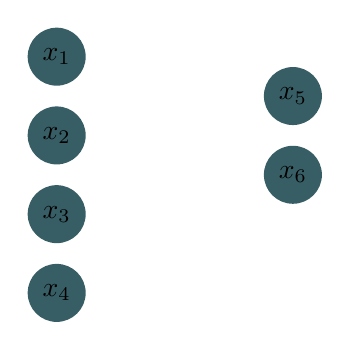
\begin{tikzpicture}[arrow/.style={thick,->,black},
            set name/.style={font=\color{myblue}\tiny\bfseries\sf},
            set/.style={ultra thick, myblue},
            every node/.style={circle},
            font=\sf
         ]
      \node[fill=myblue] (x1) at (1.0, 3.0) {$x_1$};
      \node[fill=myblue] (x2) at (1.0, 2.0) {$x_2$};
      \node[fill=myblue] (x3) at (1.0, 1.0) {$x_3$};
      \node[fill=myblue] (x4) at (1.0, 0.0) {$x_4$};
      \node[fill=myblue] (x5) at (4.0, 2.5) {$x_5$};
      \node[fill=myblue] (x6) at (4.0, 1.5) {$x_6$};


   \end{tikzpicture}
\end{figure}

\begin{proposition}[$\sufficesAlg{G}$ Computes $\sufficesR_{G}$]
   \label{prop:sufficesAlg-computes-suffices}
   For any dependence graph $G$, any $X \subseteq \sources{G}$ and any $Y \subseteq \sinks{G}$ we have:
   \[X \sufficesAlg{G} Y \iff \sufficesR_{g}(X) = Y\]
\end{proposition}
\begin{proof}
   See \apdxsecref{apdx:suffices-alg}.
\end{proof}

\subsubsection{Derived algorithms}

\proprefTwo{demandedByAlg-computes-demandedBy}{sufficesAlg-computes-suffices} justify treating
$\demandedByAlg{G}$ and $\sufficesAlg{G}$ as functions. Using \lemref{conjugate:image-preimage-duality} we can
define a direct algorithm for $\demandsR_{G}$ from $\demandedByAlg{G}$ by simply flipping the graph, and the
same can be done to acquire an algorithm for $\preimageDualR_{G}$ from $\sufficesAlg{G}$. Using
\lemref{conjugate:image-preimage-duality} and \defref{conjugate:de-morgan-dual} we can also define alternative
algorithms for all 4 operators using the De Morgan dual construction. These are summarised in the table below.

\begin{figure}
\begin{tabular}{|c|l|l|c|c|}
\emph{Abstract operator} & \emph{Direct algorithm} & \emph{De Morgan Dual algorithm} \\
$\demandedByR_{G}$ & $\demandedByAlg{G}$ & $\dual{\sufficesAlg{\opGraph{G}}}$ \\
$\demandsR_{G}$ & $\demandedByAlg{\opGraph{G}}$ \\
$\sufficesR_{G}$ & $\sufficesAlg{G}$ \\
$\preimageDualR_{G}$ & $\sufficesAlg{\opGraph{G}}$
\end{tabular}
\caption{Direct and De Morgan Dual implementations of all 4 operators}
\end{figure}


\noindent In \secref{evaluation} we contrast the performance of the direct and De Morgan dual implementations
of $\demandedByR_{G}$, used to implement linked inputs/outputs as shown in \secref{introduction}.

\subsection{$\relInputR_G$ and $\relOutputR_G$ for Dependence Graphs}

Now we can provide a formal account of the notions of linked inputs and outputs.

\begin{definition}[Linked inputs and outputs]
   For a dependence graph $G$ let:
   \begin{enumerate}
      \item $\relInputR_{G} \eqdef \demandsR_{G} \after \demandedByR_{G}$\hfill (linked inputs)
      \item $\relOutputR_{G} \eqdef \demandedByR_{G} \after \demandsR_{G}$\hfill (linked outputs)
   \end{enumerate}
\end{definition}

Intuitively, linked outputs and linked inputs are relations of \emph{cognacy} (common ancestry) in $G$ and
$\opGraph{G}$ respectively. For a set of inputs $X \subseteq \sources{G}$, linked inputs asks ``what other
inputs are demanded by the outputs which demand X?''; it first finds all outputs $\demandedByR_{G}(X)$ that
our inputs are demanded by, and then computes the inputs that those outputs demand,
i.e.~$\demandsR_{G}(\demandedByR_{G}(X'))$. Conversely for a set of outputs $Y \subseteq \sinks{G}$, linked outputs asks
``what other outputs demand the inputs that Y demands''; it first finds all inputs $\demandsR_{G}(Y')$ that
our outputs demand, and then computes the outputs that those inputs $\demandsR_{G}(Y)$ demand,
i.e.~$\demandedByR_{G}(\demandsR_{G}(Y))$.

% In general, neither $\relInputR_{G}$ nor $\relOutputR_{G}$ is inflationary; inputs which are not used anywhere
% are not preserved by the $\relInputR_{G}$ round-trip, and outputs which don't require any inputs are not
% preserved by the $\relOutputR_{G}$ round-trip. Thus in general we have neither $X' \subseteq
% \relInputR_{G}(X')$ nor $X' \subseteq \relOutputR_{G}(X')$. However if we constrain things so that there are
% no inputs which are unused, then $\demandsR_G$ will preserve $\bot$, i.e.~$\demandsR_G(\emptyset) =
% \emptyset$, and $\relOutputR_{G}$ will preserve the original output selection. Similarly, if we constrain
% things so that all outputs demand some input, then $\demandedByR_G$ will preserve $\bot$, and $\relInputR_{G}$
% will preserve the original input selection:

% \begin{lemma}
% \item
% \begin{enumerate}
%    \item If $\demandedByR_G(\emptyset) = \emptyset$, then for all $X$ we have $\relInputR_{G}(X) \geq X$.
%    \item If $\demandsR_G(\emptyset) = \emptyset$, then for all $Y$ we have $\relOutputR_{G}(Y) \geq Y$.
% \end{enumerate}
% \end{lemma}

% As an easy corollary, if $\demandsR_G$ and $\demandedByR_G$ both preserve $\emptyset$ then in fact they form
% an anti-tone Galois connection. In practical terms, it is possible to use this to produce a filtered view, only
% showing inputs that are actually used in a program.

% \subsubsection{Focused queries}
%
% \todo{If we want to keep this then some work required to contextualise.} We are often only interested in some
% domain-restriction of the environment $\Gamma' \subseteq \Gamma$. Happily, domain restriction of maps induces
% a pair of conjugate functions: one of them maps the unselected part of the environment ($\Gamma \setminus
% \Gamma'$) to $\top$, and the other  maps the unselected values to $\bot$. In practical terms, this mechanism
% could be used to allow for ``focused'' queries -- the ability to restrict the parts of the output or input
% that the user is interested in using to mediate the linked inputs or outputs query.
